\section{La vie en Inde...}

Date: 08/02/2008

\begin{multicols}{2}

Nous revoici pour la suite de notre voyage... Nous sommes depuis trois jours à Jaipur, capitale du Rajasthan. Nous avons principalement fait des visites à pieds, nous sommes baladés dans des bazaars en particulier dans la vieille ville, qu'on appelle la ville rose. Puis nous avons rencontré Raj, un jeune qui aide les enfants des rues en leur apprenant la musique, l'anglais, les maths. A la base c'est un artiste, son métier est de faire des spectacles de marionnettes dans des grands hôtels. Nous avons passé une journée complête avec lui et les enfants, il nous a expliqué son projet de construire une école prochainement. C'était impressionnant de voir comment les enfants le considéraient comme leur père. En fait c'est un grand enfant que nous avons rencontré, qui essaie d'aider les autres. Nous essaierons de lui envoyer des fournitures scolaires ainsi que d'autres choses pouvant lui être utiles quand nous rentrerons, avis aux bons coeurs. Entre nos multiples balades dans Jaipur nous avons ensuite visité le palais du vent (Hawa Mahal), façade aux multiples fenêtres destinées autrefois à permettre aux femmes du harem de voir les festivités dans la rue sans être vues. Ensuite nous avons vu le fort de Amber, perché sur une colline dans un cadre magnifique. Les multiples styles architecturaux et la vue depuis le haut nous ont encore fait de beaux souvenirs. En tout cas une chose est sûre, l'Inde nous dépayse complètement et l'on découvre ici plein de choses magnifiques. Jamais vu tant de merveilles au kilomètre carré, qu'il s'agisse des monuments, des rues ou des gens. Chaque journée est riche en émotions. Mais il faut savoir que vivre ici nécessite un temps d'adaptation ainsi qu'une capacité à prendre du recul. En effet, la première chose à savoir est que ici tout se passe dans la rue. Les vendeurs y ont leurs échoppes, les rickshaws, taxis, cyclopouss, motos, voitures, camions, vaches et piétons s'y pressent pêle-mêle, mais surtout les gens y vivent. Enfants à moitié nus, veillards édentés, pères de famille vivent à même le trottoir, sur des couvertures ou sur des charettes. On ne marche donc pas sur le trottoir, par contre on marche sur la route et chacun va où il veut, à ceux de derrière de faire attention. Les bords de route servent aussi de décharge publique. Ici pas de poubelles, on jette tout devant sa porte, et on pousse jusqu'à celle du voisin.

La poussière est omnipresente, le bruit est quasi insupportable de jour comme de nuit. Le klaxon remplace le clignotant et chacun fait ce qu'il veut sans se soucier de l'autre, comme hurler dans la rue à 3h du mat ou jouer du drum à cote de quelqu'un qui dort (et quand on a une chambre dont les fenêtres ne ferment pas, on peut vous dire que c'est pas très tranquille les nuits). Le temps est une notion toute relative ici, de même que la propreté. La cuisine des petits restaurants est dehors, sur le trottoir, sans murs ni aucune protection, les cafards se baladent sur les murs sans complexes, les chambres d'hôtel sont poussiéreuses, les salles de bain heu... bof. Mais pour nous pas de soucis, on n'y prête plus vraiment attention. Et les animaux, partout il y en a, pour nous c'est incroyable. Outre les vaches sacrées qui se baladent sur les routes et que les voitures évitent soigneusement, de nombreux chiens et chèvres vivent dans la rue. On trouve aussi beaucoup de poules, de singes, d'écureuils, d'oiseaux. Les rats eux préfèrent quand même les gares aux rues, c'est déjà ça.

La nourriture, c'est aussi quelque chose. Très bon, mais très épicé. On a par contre un peu de mal à s'y faire et on commence à reprendre des habitudes alimentaires occidentales : le riz presque nature pour tenir au ventre, le coca pour aider à la digestion et boire autre chose que de l'eau purifiée aux pastilles, les oeufs au plat et beurre confiture au ptit dej, les chips Lays pour le coup de faim et ce midi, le Mac Do. Tant d'autres choses à raconter, mais le principal est déjà dit et permet de brosser l'atmosphàre générale, car la vie ici se vie évidemment bien au delà de nos visites touristiques. Ah oui, encore une chose trèèès importante ici : les arnaques ! 100% du temps les gens cherchent à nous arnaquer, alors il faut savoir déjouer les pièges, et surtout ne jamais faire totalement confiance et toujours anticiper. Evidemment, il y a les prix qu'il faut marchander, mais aussi les rickshaws qui nous arrêtent où ils veulent pour avoir du backchich à la boutique ou nous faire acheter des légumes pour faire de la monnaie. Les offices de tourismes ou bureaux de tourisme en tout genre envoient vers des hôtels hors de prix ou vendent des tickets de train trois fois leur valeur. Les boss des hôtels nous montrent la chambre la plus pourrie d'une gamme pour que l'on prenne la gamme au dessus, les gentilles personnent qui aiment bien les francais et demandent à ce qu'on traduise une lettre de remerciement en Français sont invariablement commercants... impossible d'écrire toutes les arnaques auxquelles on a droit, mais tout ça pour dire que c'est pas de tout repos. Cela dit, les enfants qui viennent nous voir sont juste fiers et heureux de pouvoir nous dire "hello, what is your name, how are you" en nous serrant la main et nous font des sourires magnifiques. On nous aborde souvent juste par curiosité "From which country ? Oh France, so you are from Parissssse ?"

\hspace*{-0.65cm}
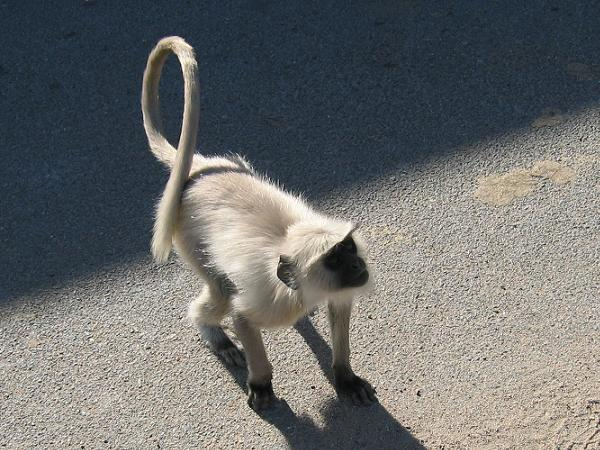
\includegraphics[width=4.8cm]{articles/La-vie-en-inde/singe.jpg}
Un macaque

Allez les gens, à la prochaine

\end{multicols}
